\chapter{Temporal Analysis of the Design and Development of Mobile Applications}
\label{ch:findings_chapter}
Sieveable enabled retrieving a sample of apps across multiple search criteria to meet a diverse set of search goals.
In this chapter, I present illustrative temporal analysis examples to understand how apps are evolved over time.

\section{Visual Design Mining}

Mobile UI design is always evolving and new guidelines are put into place to create a consistent experience across the platform.
For instance, Google introduced Material Design, a design language that makes use of elements from print design, responsive transitions, and depth effects \cite{Google_Material_Design}.
Google announced the main concepts of the design language on June 25, 2014.
Since then several third-party implementations have been introduced and used by developers.
A year later, Google introduced an official library called the Android Design Support Library, which allows developers to implement a number of material design components that are backward compatible with old devices.
We can use Sieveable to find apps that use specific material design components and find when they were adopted by developers.
We can also aggregate the results by download count and find trends in implementing them among popular and less popular apps.

\subsection{Material Design Components}
In this section, I present a set of analyses on the adoption rate of three major material design components over time.

\subsubsection{Floating Action Button}
\begin{figure}[H]
	\centering
	{{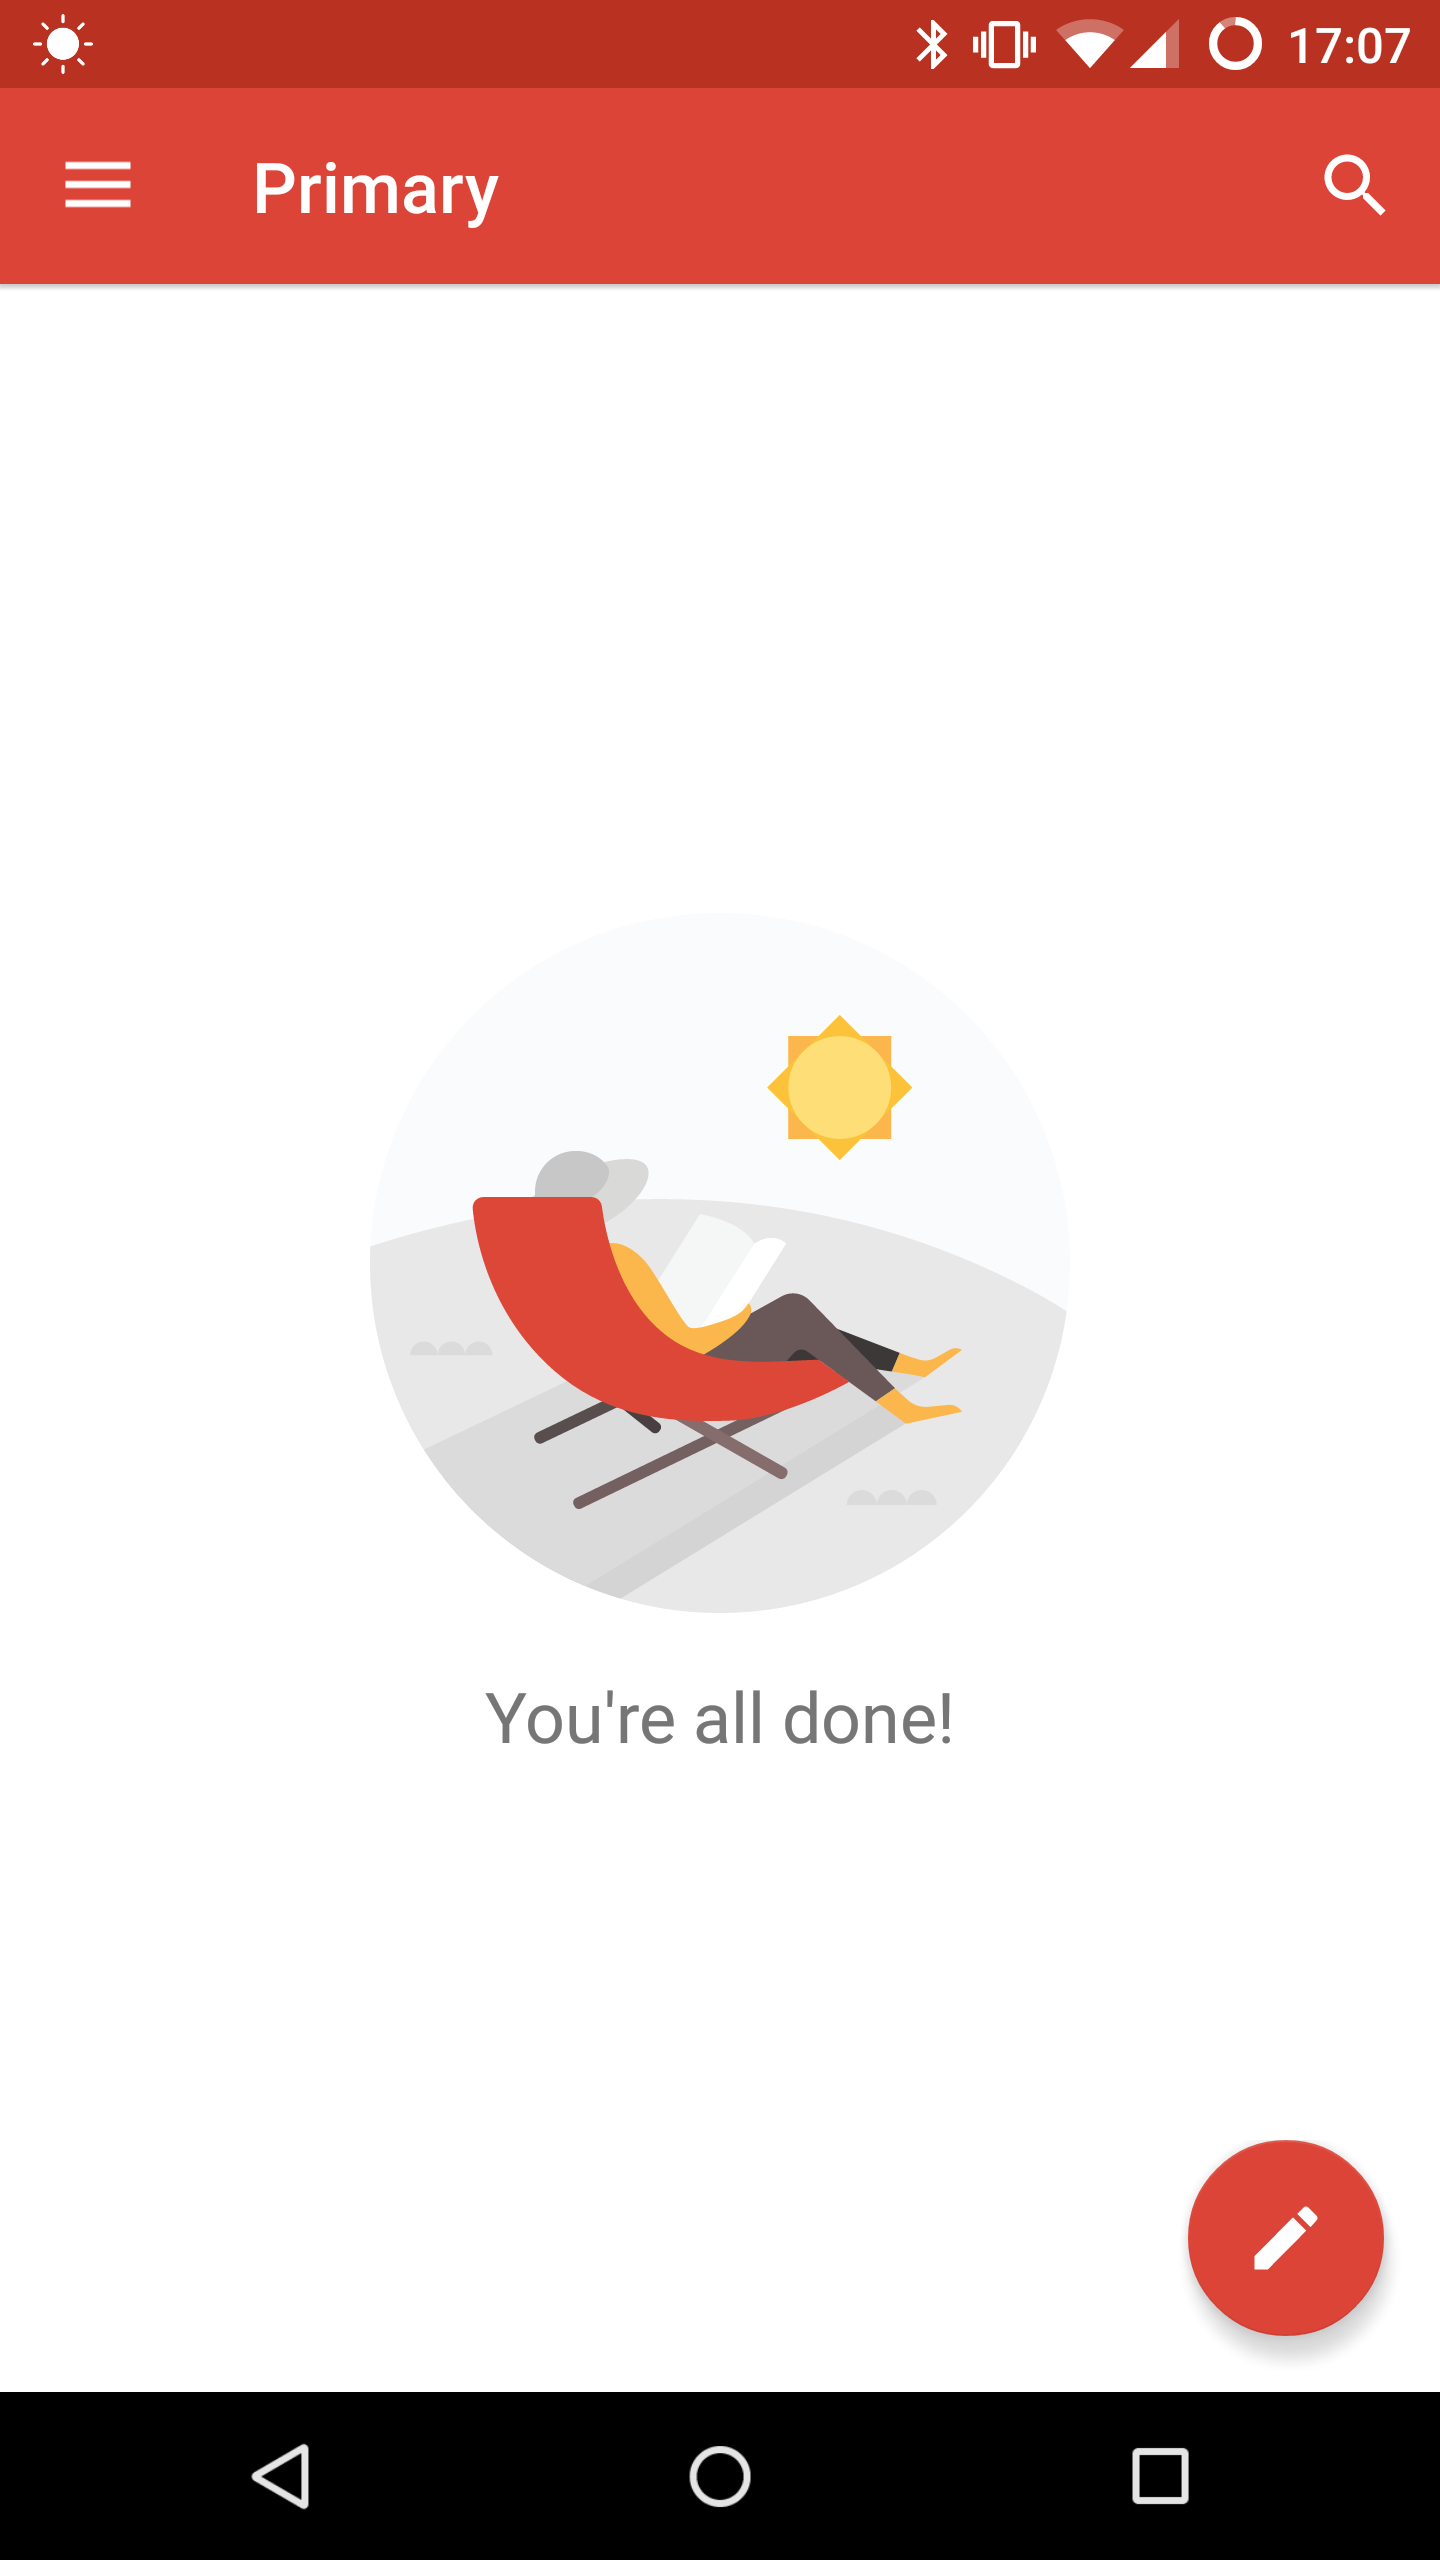
\includegraphics[scale=0.1]{figures/findings/fab-Gmail.png} }}%
	\qquad
	{{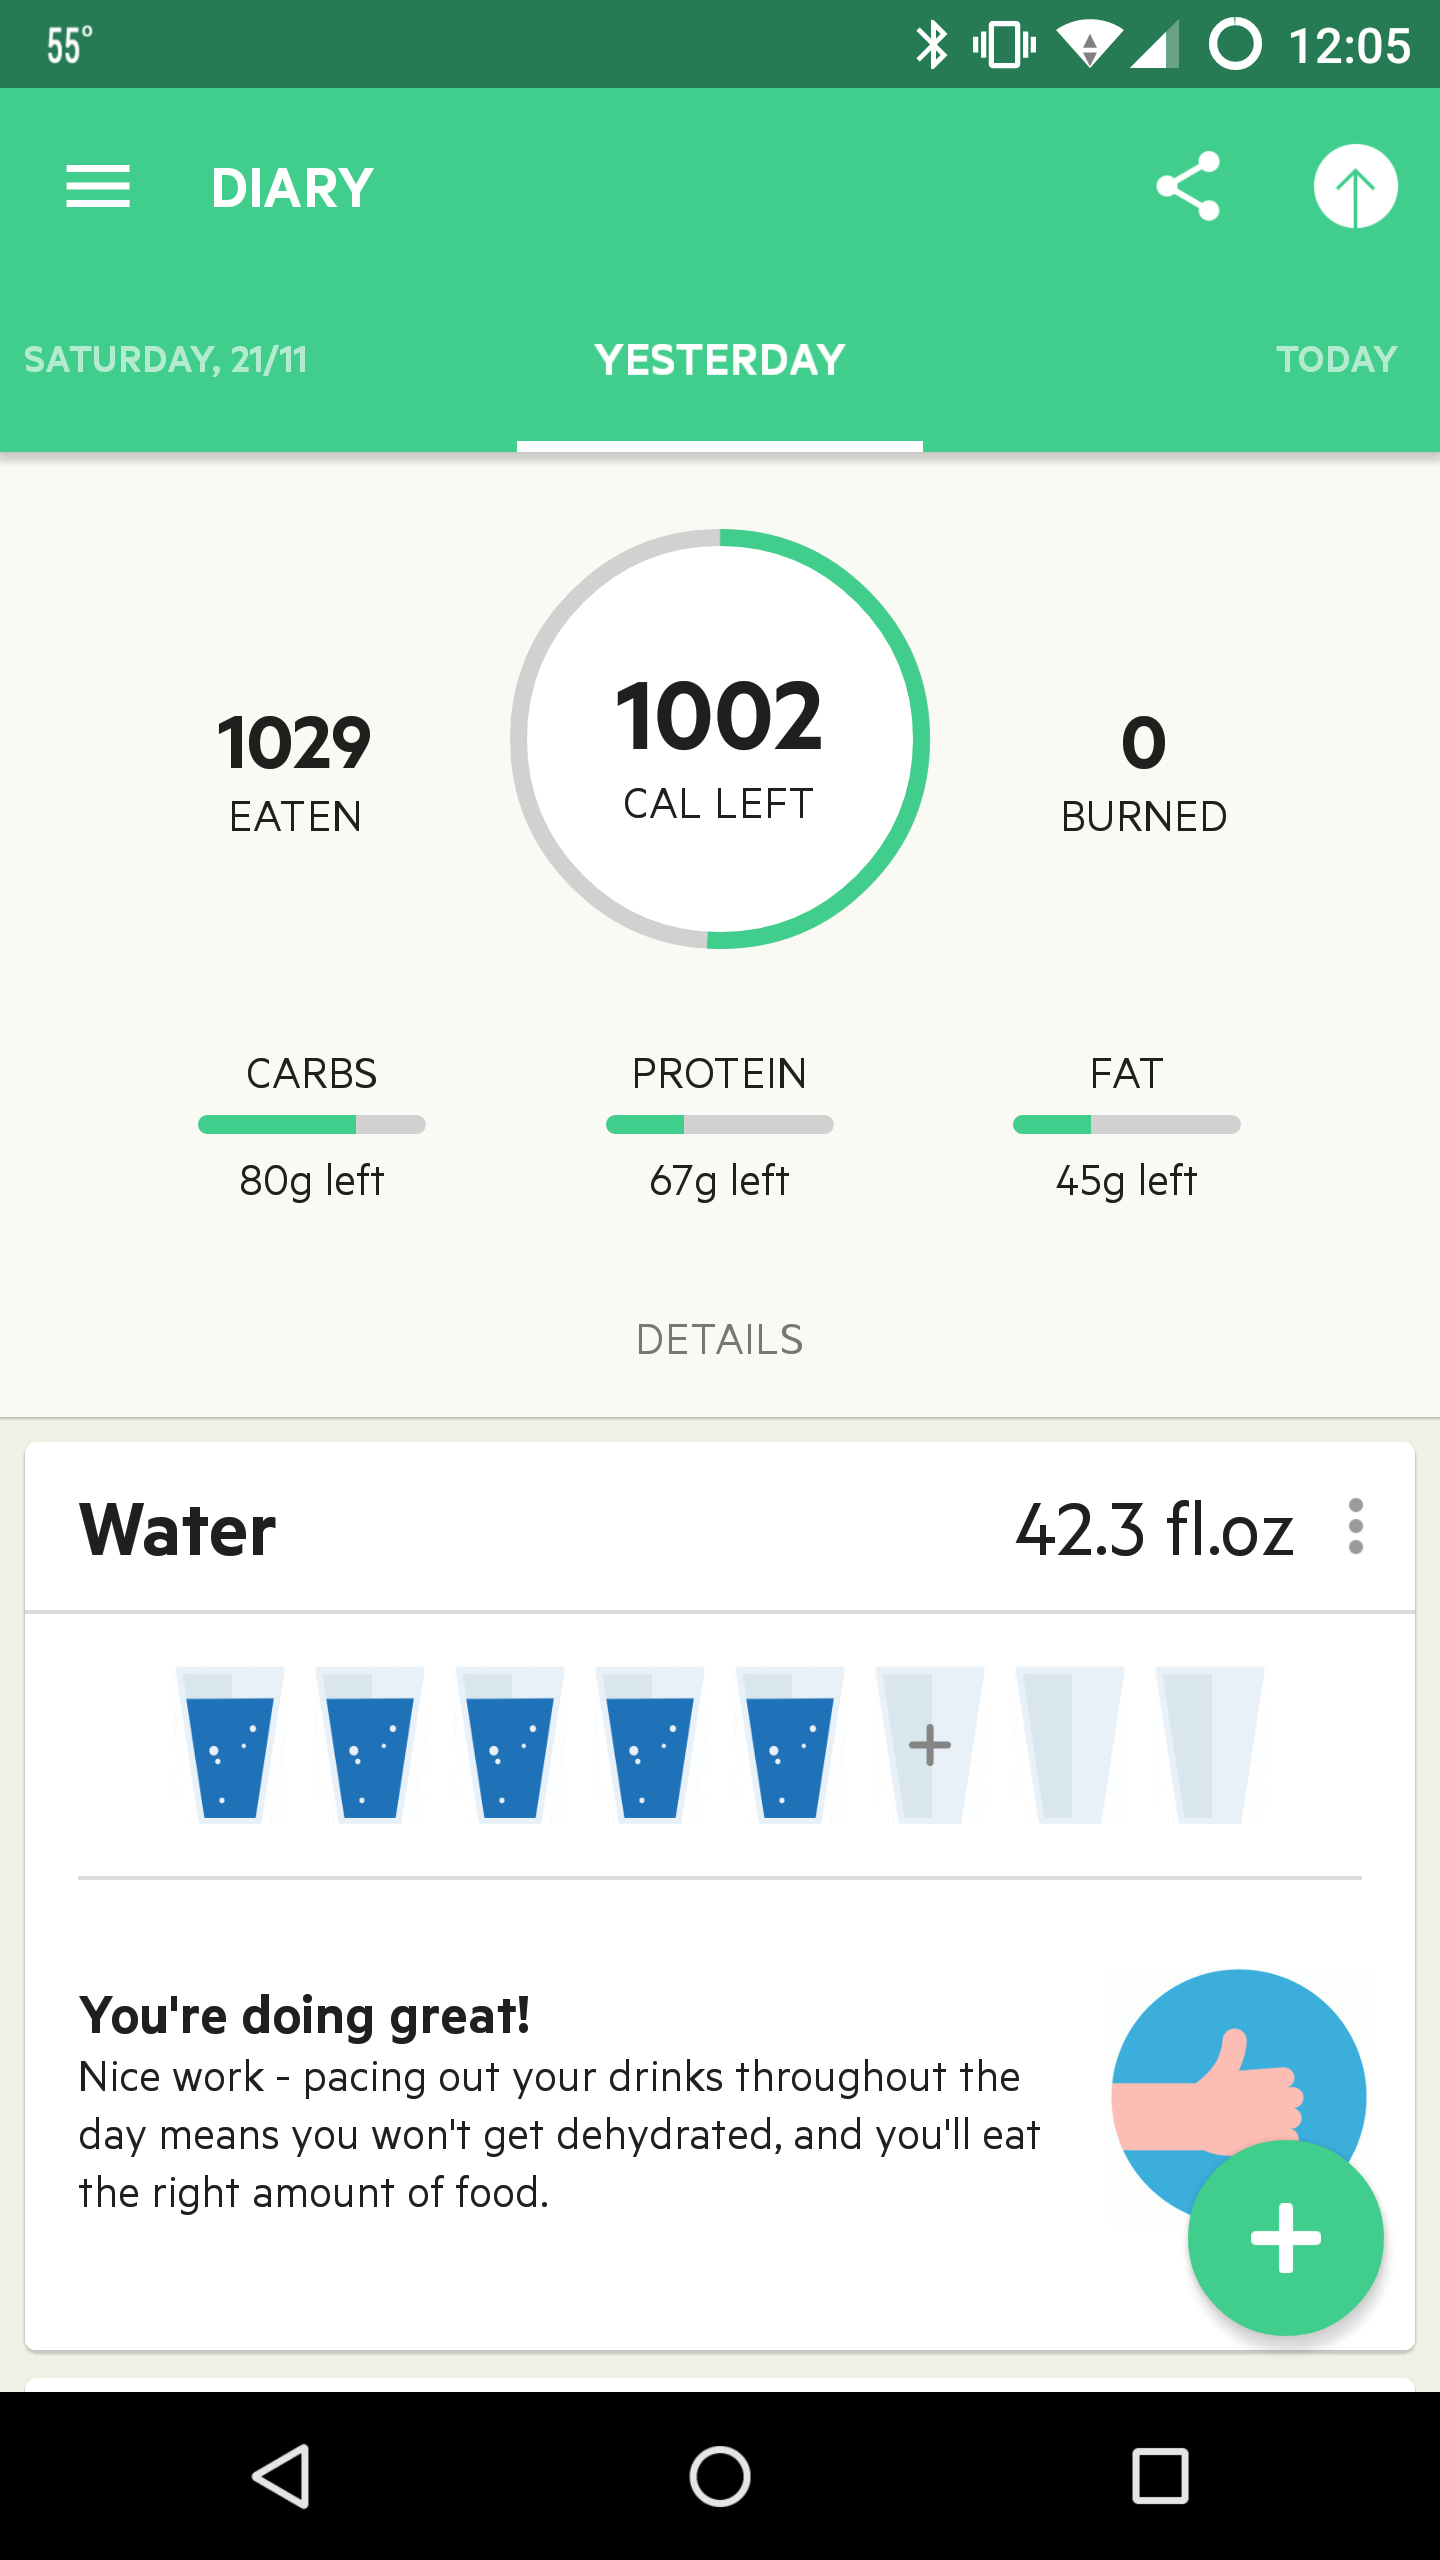
\includegraphics[scale=0.1]{figures/findings/fab-lifesum.png} }}%
	\caption{The Floating Action Button (FAB) shown at the bottom right corner of two apps, Gmail and Lifesum}%
	\label{fig:figure_fab_screenshot}
\end{figure}
The Floating Action Button (FAB) is a circled button floating above the UI to promote the primary action in the app (Figure~\ref{fig:figure_fab_screenshot}).
While developers can create a custom FAB with material design style, there are a few libraries that simplify adding this widget.
We can use Sieveable to aid developers and make an informed decision of using a specific library over other alternatives.
With Sieveable, one can examine the popularity of a specific UI library within any time window.
This can provide insightful feedback to UI framework engineers or developers on how well the components they developed are received by third-party developers.
We can find the trends of adopting the FAB as a design pattern over time using different alternatives.
At the time of writing, there are four alternative ways to implement the FAB in Android: the official design support library \cite{Android_Design_Support_Lib}, and three other additional third-party libraries \cite{android-floating-action-button, FloatingActionButton, fab}.
I use the following sieveable queries to retrieve the set of apps that implement the FAB using the previously mentioned libraries: 

\begin{minted}[fontsize=\small]{xml}
MATCH app
WHERE
<android.support.design.widget.FloatingActionButton />
<date-published>(*)</date-published>
<rating>(*)</rating>
<downloads>(*)</downloads>
RETURN app, l$1 AS rDate, l$2 as rating, l$3 as downloads

MATCH app
WHERE
<com.getbase.floatingactionbutton.FloatingActionButton />
<date-published>(*)</date-published>
<rating>(*)</rating>
<downloads>(*)</downloads>
RETURN app, l$1 AS rDate, l$2 as rating, l$3 as downloads

MATCH app
WHERE
<com.melnykov.fab.FloatingActionButton />
<date-published>(*)</date-published>
<rating>(*)</rating>
<downloads>(*)</downloads>
RETURN app, l$1 AS rDate, l$2 as rating, l$3 as downloads

MATCH app
WHERE
<com.software.shell.fab.ActionButton />
<date-published>(*)</date-published>
<rating>(*)</rating>
<downloads>(*)</downloads>
RETURN app, l$1 AS rDate, l$2 as rating, l$3 as downloads
\end{minted}


When we combine all the results together and aggregate by the release year in which the first adoption is observed, we can get a sense of the adoption rate of the FAB over the last years Figure~\ref{fig:figure}.

This shows that the adoption rate of this design pattern is growing slowly since it was first introduced in June 2014.
We can also analyze the adoption rate of the different implementation or libraries options over time.
In Figure~\ref{fig:figure}, we can see that apps started adopted this pattern before the official release.
Once an official library was introduced by Google in May 2015 \cite{}, the adoption rate started to increase noticeably.
This suggests that a small number developers tend to use third-party libraries to implement a new design that is not yet officially supported.
The larger number of developers, however, are much quicker to use a consistent implementation by an official library.

\section{Accessibility Mining Analysis}

\section{Security Mining Analysis}
